
%\documentclass[10pt]{phdsymp} %!PN
\documentclass[9pt, twocolumn]{phdsymp} %!PN
%\documentclass[12pt,draft]{phdsymp} %!PN
%\documentstyle[twocolumn]{phdsymp}
%\documentstyle[12pt,twoside,draft]{phdsymp}
%\documentstyle[9pt,twocolumn,technote,twoside]{phdsymp}

\usepackage[english]{babel}       % Voor nederlandstalige hyphenatie (woordsplitsing)

\usepackage{graphicx}                   % Om figuren te kunnen verwerken
\usepackage{graphics}			% Om figuren te verwerken.
\graphicspath{{figuren/}}               % De plaats waar latex zijn figuren gaat halen.

\usepackage{times}

\hyphenation{si-mu-la-ted re-a-lis-tic packets really in-clu-ding}

\def\BibTeX{{\rm B\kern-.05em{\sc i\kern-.025em b}\kern-.08em
    T\kern-.1667em\lower.7ex\hbox{E}\kern-.125emX}}

\newtheorem{theorem}{Theorem}

\begin{document}

\title{Identifying experts through a framework for knowledge extraction from public online sources} %!PN

\author{Simon Buelens and Mattias Putman}

\supervisor{Prof. Dr. Ir. Filip De Turck, Dr. Ir. Elena Tsiporkova, Dr. Ir. Tom Tourw\'e, Ir. Anna Hristoskova, Ir. Tim Wauters}

\maketitle

\begin{abstract} 


\end{abstract}

\begin{keywords}
author disambiguation, semantic web, information processing, clustering
\end{keywords}

\section{Introduction}


\section{Framework}

\begin{figure}
\centering
%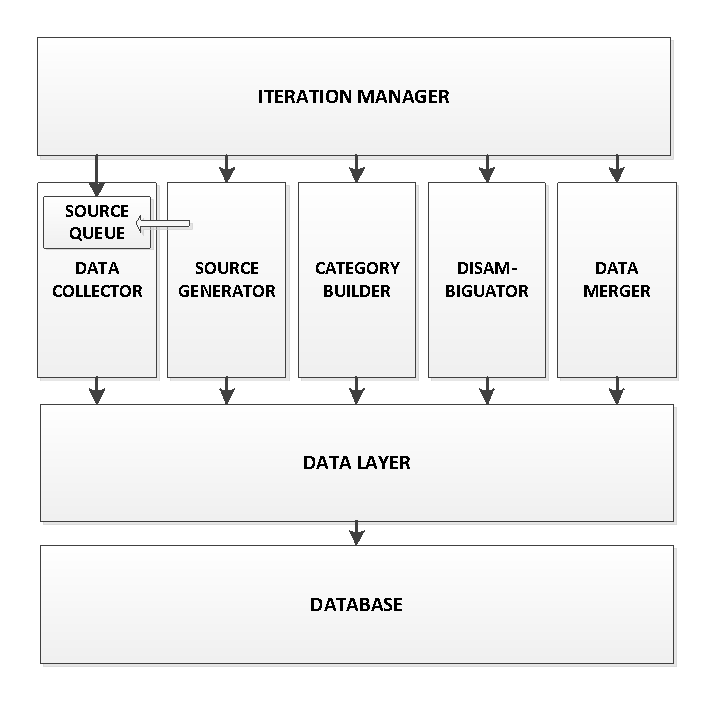
\includegraphics[width= 0.35\textwidth]{fig/architectuur.pdf}
\caption{Service Manager}
\label{fig:architectuur}
\end{figure}

%\begin{description}
%\item[- Service Interaction Manager] Serves as a regulator for interactions with other parts of the system (AI and Context Manager) and external services.
%\item[- Service Discovery] An interface offering classic syntax based service discovery. This component is responsible for finding semantic devices and their matching services and invoking and monitoring the semantically described services. 
%\item[- MatchMaker] A service for matching incoming semantic requests with the descriptions of the services in the local repository. This component communicates with the \textit{Context Manager} in order to take into account the current context. A simple lightweight matchmaker was implemented supporting matching based on inputs, outputs, preconditions and effects, and including the local context into the process. 
%\item[- Service Repository] This component is responsible for checking the availability of the offered services and provide a list of currently available services to the \textit{MatchMaker}. Services that are composed out of other services can rely on devices on the network for offering some subcomponent, when these are not available, the composite service will not be advertised by the \textit{Service Repository} as available.
%\item[- Service Execution Manager] The best suitable service out of the obtained matching results, is selected by this component. The selection can be based on how well the offered services matches the semantic requests, but also on context information such as the distance to a goal location. After selecting a service, the semantic inputs are transformed according to the grounding and the service is invoked. The results of the service invocation are then translated to semantic outputs. Another task of this component is the monitoring of the progress of execution. When the execution of the service fails, the \textit{Execution Manager} is informed of this fact by the eventing mechanism and the next best service in the list will be selected for execution.
%\end{description}


\section{Technology study}


\begin{figure}[htpb!]
\centering
%\includegraphics[width= 0.35\textwidth]{fig/abstract_ontologie.pdf}
\caption{Top-level of robot ontology}
\label{fig:ontology}
\end{figure}

\section{Testresults}

\begin{figure}[htpb!]
\centering
%\includegraphics[width= 0.4\textwidth]{fig/performance_total.pdf}
\caption{Performance test of the matchmaker on Laptop (2GHz processor, 1GB RAM) and ALIX (500MHz processor, 256MB RAM)}
\label{fig:testperformance}
\end{figure}


\begin{figure}[htpb!]
\centering
%\includegraphics[width= 0.4\textwidth]{fig/parameters_en.pdf}
\caption{Test of influence of parameters on performance on Laptop (2GHz processor, 1GB RAM)}
\label{fig:testparameters}
\end{figure}



\section{Conclusions and future work}


%\nocite{*}
\bibliographystyle{phdsymp}
%%%%%\bibliography{bib-file}  % commented if *.bbl file included, as
%%%%%see below


%%%%%%%%%%%%%%%%% BIBLIOGRAPHY IN THE LaTeX file !!!!! %%%%%%%%%%%%%%%%%%%%%%%%
%% This is nothing else than the phdsymp_sample2e.bbl file that you would%%
%% obtain with BibTeX: you do not need to send around the *.bbl file        
%%
%%---------------------------------------------------------------------------%%
%
\begin{thebibliography}{1}
%\bibitem{paper}
%Bart Lannoo, Didier Colle, Mario Pickavet, Piet Demeester,
%\newblock {\em Optical Switching Architecture to Implement Moveable Cells in a Multimedia Train Environment},
%\newblock Proc. of ECOC 2004, 30th European Conf. on Optical Communication, vol. 3, pp. 344-345, Stockholm, Sweden, 5-9 Sep. 2004.
%
\bibitem{upnp}
Donoho A, Costa-requena J, Mcgee T, Messer A, Fiddian-green A, Fuller J. \newblock{\em UPnP Device Architecture 1.1.} Oct. 2008. 

\bibitem{cling}
Bauer C. \newblock{\em Cling UPnP.} 22 Mar. 2011. Available from: http://teleal.org/projects/cling/

\bibitem{owl}
Smith M, Welty C, McGuinness D. \newblock{\em OWL - Web Ontology Language.} 5 Apr. 2011. Available from: http://www.w3.org/TR/owl-guide/

\bibitem{owls}
Martin D, Burstein M, Hobbs J, Lassila O, McDermott D, McIlraith S, et al. \newblock{\em OWL-S - Semantic Markup for Web Services.} 21 Sep. 2010. Available from: http://www.w3.org/Submission/OWL-S/

\bibitem{owlstc}
SemWebCentral. \newblock{\em OWL-S Service Retrieval Test Collection: Project Info.} May 16 May. 2011. Available from: http://www.semwebcentral.org/projects/owls-tc/



%
%\bibitem{click}
%\newblock {\em The Click Modular Router Project},
%\newblock http://www.read.cs.ucla.edu/click/
%
%\bibitem{ns}
%\newblock {\em {NS} -- {N}etwork {S}imulator},
%\newblock http://nsnam.isi.edu/nsnam/
\end{thebibliography}
%
%%---------------------------------------------------------------------------%%

\end{document}

%%%%%%%%%%%%%%%%%%%%%  End of phdsymp_sample2e.tex  %%%%%%%%%%%%%%%%%%%%%%%%%%%
